\chapter{Liveness analyse}

\section{Control Flow Graphs}
Een \textbf{Control Flow Graph (CFG)} is een niet-lineaire voorstelling van de assemblycode die uitgevoerd wordt. Elke instructie wordt een knoop in de CFG.

\begin{figure}[ht]
	
	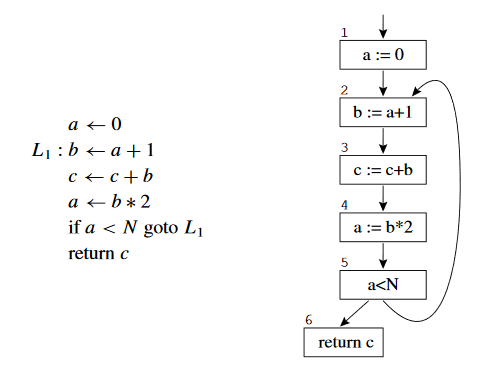
\includegraphics[width=\textwidth]{cfg_example}
	\caption{De CFG van een programma.}
	\label{fig:cfg_example}
\end{figure}


\QA{Hoeveel registers zijn er nodig om de temporaries $a$, $b$ en $c$ bij te houden voor het programma in figuur \ref{fig:cfg_example}? De variabele $c$ is een parameter die meegegeven wordt aan de functie.}{
Eerst afvragen waar in het programma de waarde van deze variabelen een rol kunnen spelen. 
}

Voor de variabele $a$ kan nagegaan worden waar de waarde nodig is. Er is sprake van vijf verschillende sets:
\begin{itemize}
	\item \textbf{in set}:  De in set geeft voor instructie $x$ de variabelen die nodig zijn van instructie $x - 1$. Zo is in[2] = \{a, c\}.
	\item \textbf{out set}: De out set geeft voor instructie $x$ de variabelen die nodig zijn voor instructie $x + 1$. Zo is out[1] = \{a, c\}.
	\item \textbf{def set}: De def set geeft voor instructie $x$ de variabelen die gedeclareerd worden door instructie $x$. Zo is def[1] = \{a\}.
	\item \textbf{use set}: De use set geeft voor instructie$x$ de variabelen die gebruikt worden door instructie $x$. Zo is use[2] = \{a, b\}.
	\item \textbf{succ set}: De succesor set geeft voor instructie $x$ de instructies die op instructie $x$ kunnen volgen. Zo is succ[5] = \{2, 6\}.
\end{itemize}

Figuur \ref{fig:use_defs} toont de verschillende locaties waar de waarde van $a$ vereist is.

\begin{figure}[ht]
	\centering
	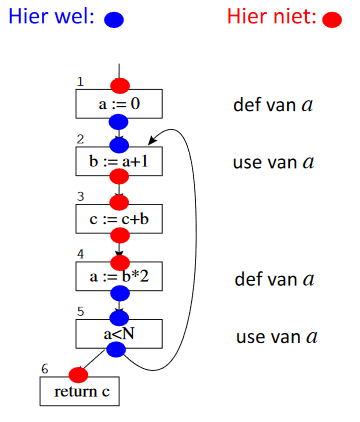
\includegraphics[width=0.5\textwidth]{use_defs}
	\caption{De plaatsen waar de waarde van $a$ een rol speelt.}
	\label{fig:use_defs}
\end{figure}

De \textbf{in} en \textbf{out} sets kunnen bekomen worden met volgende vergelijking:
\begin{align*}
	in[n] & = use[n] \cup (out[n] - def[n]) \\
	out[n] & = \bigcup_{s \in succ[n]} in[s]
\end{align*}

Via de \textbf{in} en \textbf{out} set kan de \textbf{liveness range} van elke variabele bepaald worden:
\begin{align*}
in[1] & = \{c\} \\
out[1] & = \{a, c\}\\
in[2] & = \{a, c\}\\
out[2] & = \{b, c\}\\
in[3] & = \{b, c\}\\
out[3] & = \{b, c\}\\
in[4] & = \{b, c\}\\
out[4] & = \{a, c\}\\
in[5] & = \{a, c\}\\
out[5] & = \{a, c\}\\
in[6] & = \{c\}\\
out[6] & = \{ \}
\end{align*}

Dit kan gevisualiseerd worden in de CFG (figuur \ref{fig:liveness_visual}).
\begin{figure}[ht]
	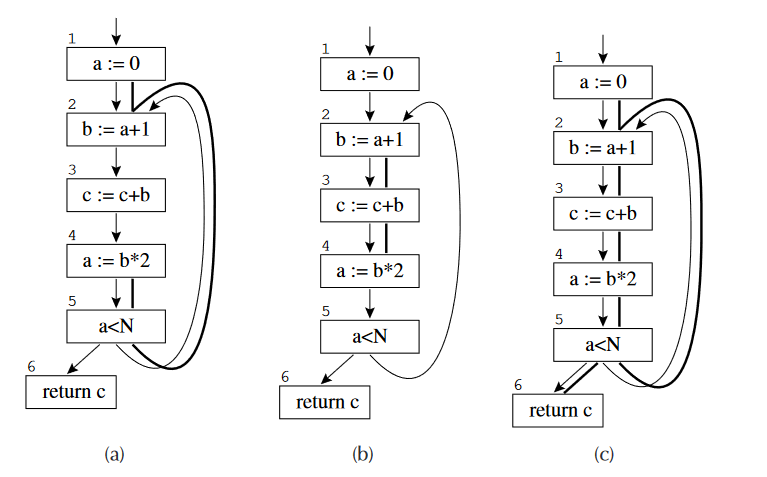
\includegraphics[width=\textwidth]{liveness_visual}
	\caption{Liveness van de variabelen $a, b$ en $c$.}
	\label{fig:liveness_visual}
\end{figure}

De vergelijking kan opgelost worden via een algoritme.
\begin{itemize}
	\item Iteratief algoritme
	\item Itereer over alle blokken in de graaf in omgekeerde volgorde (van onder naar boven).
	\begin{itemize}
		\item Maak kopie van de in en out sets
		\item Bereken de nieuwe in set
		\item Bereken de nieuwe out set
	\end{itemize}
	\item Blijf dit doen zolang er een set gewijzigd wordt.
\end{itemize}

Complexiteit:
\begin{itemize}
	\item Stel programmagrootte: $N$ statements.
	\item Elk statement kan maar 1 veranderlijke updaten, dus maximum $N$ veranderlijken.
	\item De set operatie is $O(N)$.
	\item De for loop is dan $O(N^2)$.
	\item In elke iteratie minsten 1 element toevoegen door een monotone update, dus max $2N^2$ iteraties van de repeat loop.
	\item Complexiteit: $O(N^4)$.
	\item In realiteit is het bijna lineair.
\end{itemize}

Voorstellingen van sets:
\begin{itemize}
	\item Eenvoudigste voorstelling van een set: bitvectoren. Bijvoorbeeld 64 bits, als bit 3 op 1 staat, zit 3de temporary in de s
	\item Als er te veel temporaries zijn kan gelinkte lijst gebruikt worden.
\end{itemize}


\section{Least Fixed Point \& Conservativiteit}
Er zijn meerdere oplossingen van de liveness vergelijkingen. De meest conservatieve oplossing zet alle variabelen op live bij elke instructie. 

\QA{Kan $Y$ een probleem geven? Kan $Z$ een probleem geven? (Slide 13)}{De $Y$ analyse zal nog steeds een correct programma opleveren, maar het is niet optimaal. De $Z$ analyse zal registers overschrijven.}

Een analyse is conservatief als het gedrag van het programma niet gewijzigd wordt.


\section{Statische approximatie}
Er is een verschil tussen \textbf{dynamische liveness} en \textbf{statische liveness}:
\begin{itemize}
	\item Dynamische liveness: Een variabele $a$ is dynamisch live in node $n$ als er een instructie van het programma bestaat van $n$ naar een \textit{use} van $a$ dat niet door een \textit{def} van $a$ gaat.
	\item Statische liveness: Een variabele $a$ is statisch live in node $n$ als er een pad bestaat van controle-flow verbindingen van $n$ naar een \textit{use} van $a$ dat niet door een \textit{def} van $a$ gaat.
\end{itemize}


\section{Interference Graph}
We zijn enkel geïnteresseerd welke sets meerdere veranderlijken bevat. De interference graph verbindt knopen die samen kunnen voorkomen.
\begin{figure}[ht]
	\centering
	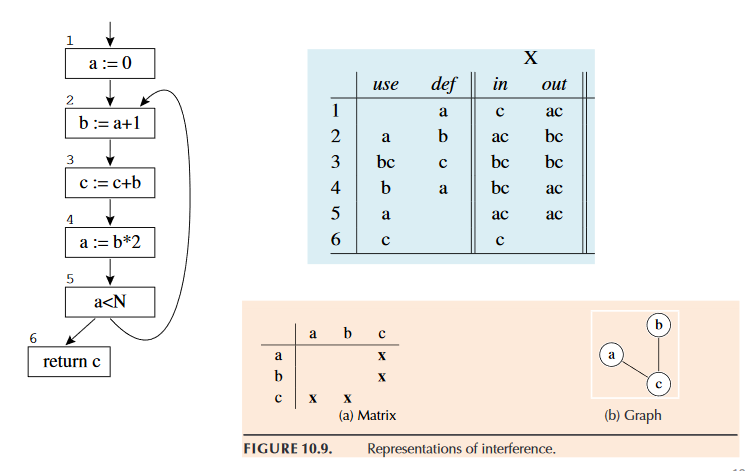
\includegraphics[width=\textwidth]{interference_graph}
\end{figure}